\documentclass[a4paper,fontset = windowsnew]{ctexbook}
\usepackage{xifthen}
\usepackage{calc}
\usepackage{graphicx}
\usepackage{tikz}
\usetikzlibrary{patterns}
%\usepackage{amsmath}
\usepackage{cexam}

\begin{document}
\chapter{基本排版程序}


%\ExplSyntaxOn
%\parindent=0pt

\begin{choices}
  1.这是选择题的题干,如
  <<
  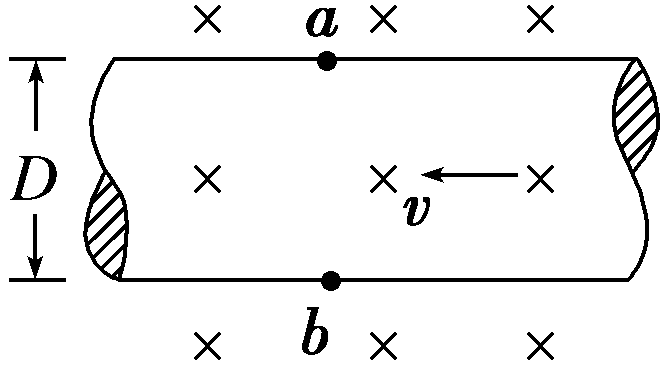
\includegraphics{1.png}
  >>
  所示是图片.其中有四个选项,分别是
  A.选项A这是长选项部分测试这是长选项部分测试这是长选项部分测试这是长选项部分测试这是长选项部分测试这是长选项部分测试这是长选项部分测试这是长选项部分测试这是长选项部分测试这是长选项部分测试这是长选项部分测试这是长选项部分测试这是长选项部分测试这是长选项部分测试
  B.选项B这是长选项部分测试这是长选项部分测试这是长选项部分测试这是长选项部分测试这是长选项部分测试这是长选项部分测试这是长选项部分测试这是长选项部分测试这是长选项部分测试这是长选项部分测试这是长选项部分测试这是长选项部分测试这是长选项部分测试这是长选项部分测试这是长选项部分测试这是长选项部分测试这是长选项部分测试
  C.选项C这是长选项部分测试这是长选项部分测试这是长选项部分测试这是长选项部分测试这是长选项部分测试这是长选项部分测试这是长选项部分测试这是长选项部分测试这是长选项部分测试这是长选项部分测试这是长选项部分测试这是长选项部分测试这是长选项部分测试这是长选项部分测试这是长选项部分测试
  D.选项D这是长选项部分测试这是长选项部分测试这是长选项部分测试这是长选项部分测试这是长选项部分测试这是长选项部分测试这是长选项部分测试这是长选项部分测试这是长选项部分测试这是长选项部分测试这是长选项部分测试这是长选项部分测试这是长选项部分测试

  a.AB

  e.这是选择题的解析部分.

  ee.这是选择题解析下一级部分,用来输入解析较长的情况.

  1.这是选择题的题干,如
  <<
  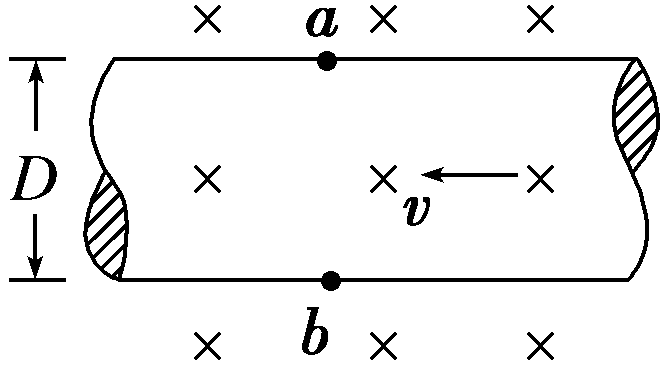
\includegraphics{1.png}
  >>
  所示是图片.其中有四个选项,分别是
  所示是图片.其中有四个选项,分别是
  所示是图片.其中有四个选项,分别是
  所示是图片.其中有四个选项,分别是
  所示是图片.其中有四个选项,分别是
  A.选项A
  B.选项B
  C.选项C
  D.选项D

  a.ABCD


\end{choices}

\end{document}
